\chapter{Physical Network Design}

\section{Devices}
\subsection{Workstations}
It is assumed that all workstations in use have been bought over from the old branch to reduce on cost. The only upgrade that would have to be made to each workstation is the installation of an SFP+ network adaptor. The recommended PCI expansion card is the \emph{ASUS 10GbE SFP+ PCIe 3.0 Network Adapter}. This recommendation is due to high reviews and a reputable manufacturer.
\subsection{Servers}
Any servers needed in the network such as email, DNS or vpn will be generic Linux based draws stored in the server room. Inside the network these servers will be placed within the DMZ area.
\subsection{Wireless Access Points (WAP)}
The Cisco Catalyst 9136 WAP has been chosen for its ability to use WiFi 6, further future-proofing our network solution.
\subsection{Media Converter}
When applicable for use the TP-Link MC220L media converter will be used to allow for use of copper cabling. An example of this use case would be the connection from switch to WAP as the WAP does not have an SFP+ port.
\subsection{Layer 3 Switch}
\subsubsection{Chassis - C4506-E}
It has been assumed that this is a switch that has been bought over from the old building to save on costs. It is an older model that is no longer sold but is going to be supported by Cisco until 2025 \parencite{cisco-4506}.
\subsubsection{Line Card - WS-X4712-SFP+E5}
This line card has been chosen because it can handle the speed of the network while being able to fit multiple in the chosen layer 3 chassis.
\begin{table}[H]
    \centering
    \begin{tabular}{|cccc|}
    \hline
    \multicolumn{1}{|c|}{SKU} & \multicolumn{1}{c|}{Ports} & \multicolumn{1}{c|}{Speed} & Connector \\ \hline
    WS-X4712-SFP+E5           & 12                         & 10GBASE-R                  & SFP+/SFP  \\ \hline
    \end{tabular}
\end{table}
\subsection{Layer 2 Switch}
\subsubsection{Chassis - C9404R}
This chassis has been chosen as it is the correct size needed to fit two supervisor cards and two line cards. This allows for the correct number of ports as well as additional for company expansion. Going any larger would not be beneficial and cost more. 
\subsubsection{Line Card - C9400-LC-48XS}
This line card has been chosen for the access layer switch as we can fit two of them in the chosen chassis. This will provide enough ports to cover the existing devices on each floor as well as any new devices bought in due to expansion.
\begin{table}[H]
    \begin{tabular}{|ccccc|}
    \hline
    \multicolumn{1}{|c|}{SKU} & \multicolumn{1}{c|}{Ports} & \multicolumn{1}{c|}{Connector} & \multicolumn{1}{c|}{Speed} & Total Needed \\ \hline
    C9400-LC-48XS             & 48                         & SFP/SFP+                       & 1/10Gbps                   & 2            \\ \hline
    \end{tabular}
\end{table}
\subsubsection{Supervisor Card - C9400-SUP-1XL-Y}
Allows for 10Gbps on each port.
\subsection{Router}
Cisco 4000 Series Integrated Services Router
\subsection{Firewall}
Cisco Firepower 4125
\section{Wiring}
A full fiber solution will be employed for this network to account for future proofing and to reduce noise on the network.
\subsection{Multimode Fiber - OM4}
The current network will be 10GBASE-SR, using OM4 fiber cables. Using OM4 fiber will give us options to expand to 40GBASE-SR or 100GBASE-SR in future also.
As the solution planned for this building is mostly copperless, OM4 cables will run between all three layers of our network model.
While the distance of 550m at 10Gbps for OM4 is overkill for a 7 story building, the allowance for higher distances at higher speeds (100m at 100Gbps) will be good for future-proofing our solution.
The cost of fiber has been decreasing steadily over the past years, due to this there will not be much of a difference between the cost of copper and fiber ethernet solutions. The only additional cost over a copper solution will be the installation of fiber network adaptors in workstation PCs.
\begin{table}[H]
    \centering
    \begin{tabular}{|ccccc|}
    \hline
    \multicolumn{1}{|c|}{\multirow{2}{*}{Designation}} & \multicolumn{4}{c|}{Distance (m)}                                                                                \\ \cline{2-5} 
    \multicolumn{1}{|c|}{}                             & \multicolumn{1}{c|}{1000BASE-SR} & \multicolumn{1}{c|}{10GBASE-SR} & \multicolumn{1}{c|}{40GBASE-SR} & 100GBASE-SR \\ \hline
    OM1                                                & 300                            & 33                              & N/A                             & N/A         \\ \hline
    OM2                                                & 600                            & 82                              & N/A                             & N/A         \\ \hline
    OM3                                                & 1000                           & 300                             & 100                             & 100         \\ \hline
    OM4                                                & 1100                           & 550                             & 150                             & 150         \\ \hline
    OM5                                                & 1100                           & 550                             & 150                             & 150         \\ \hline
    \end{tabular}
    \caption{Table of distances for Multimode Fiber cables.}
    \label{tab:fiber_distance}
\end{table}
\subsection{Uninterruptible Power Supply}

\section{Device Placement}
\subsection{Patch Pannels}
Patch pannels will be placed on each floor to house access section L2 switches. This allows for the creation of several points of failure, as opposed to a single point of failure of storing all switches in the server room.
\subsection{Ground Floor}
\begin{figure}[H]
    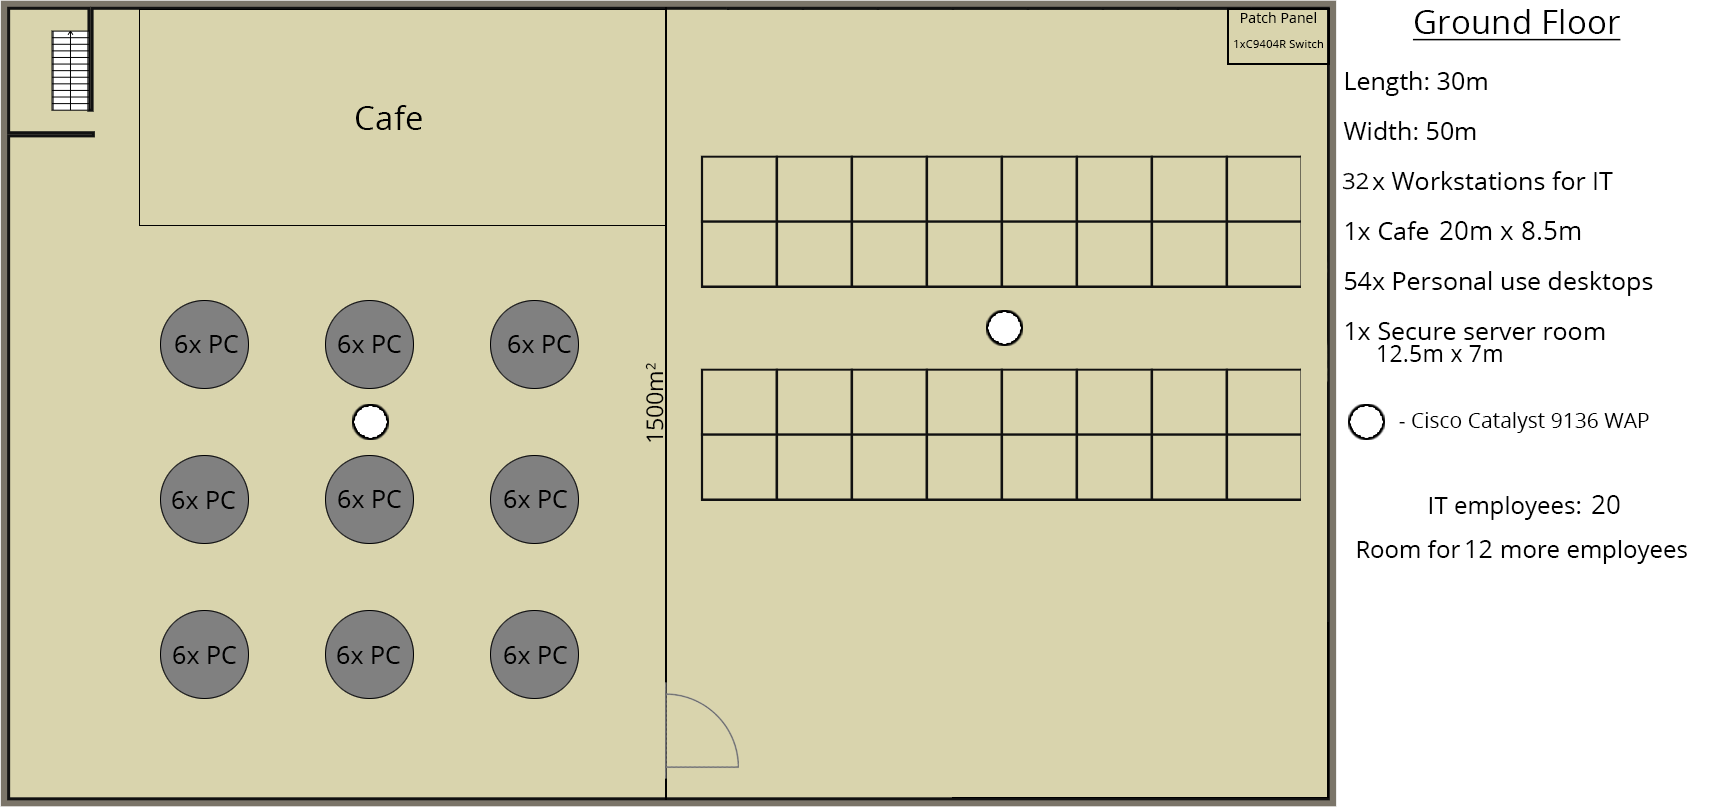
\includegraphics[width=15cm]{Figures/ground.png}
    \caption{Ground floor plan}
    \label{fig:ground_floor}
\end{figure}
\subsection{1st Floor}
\begin{figure}[H]
    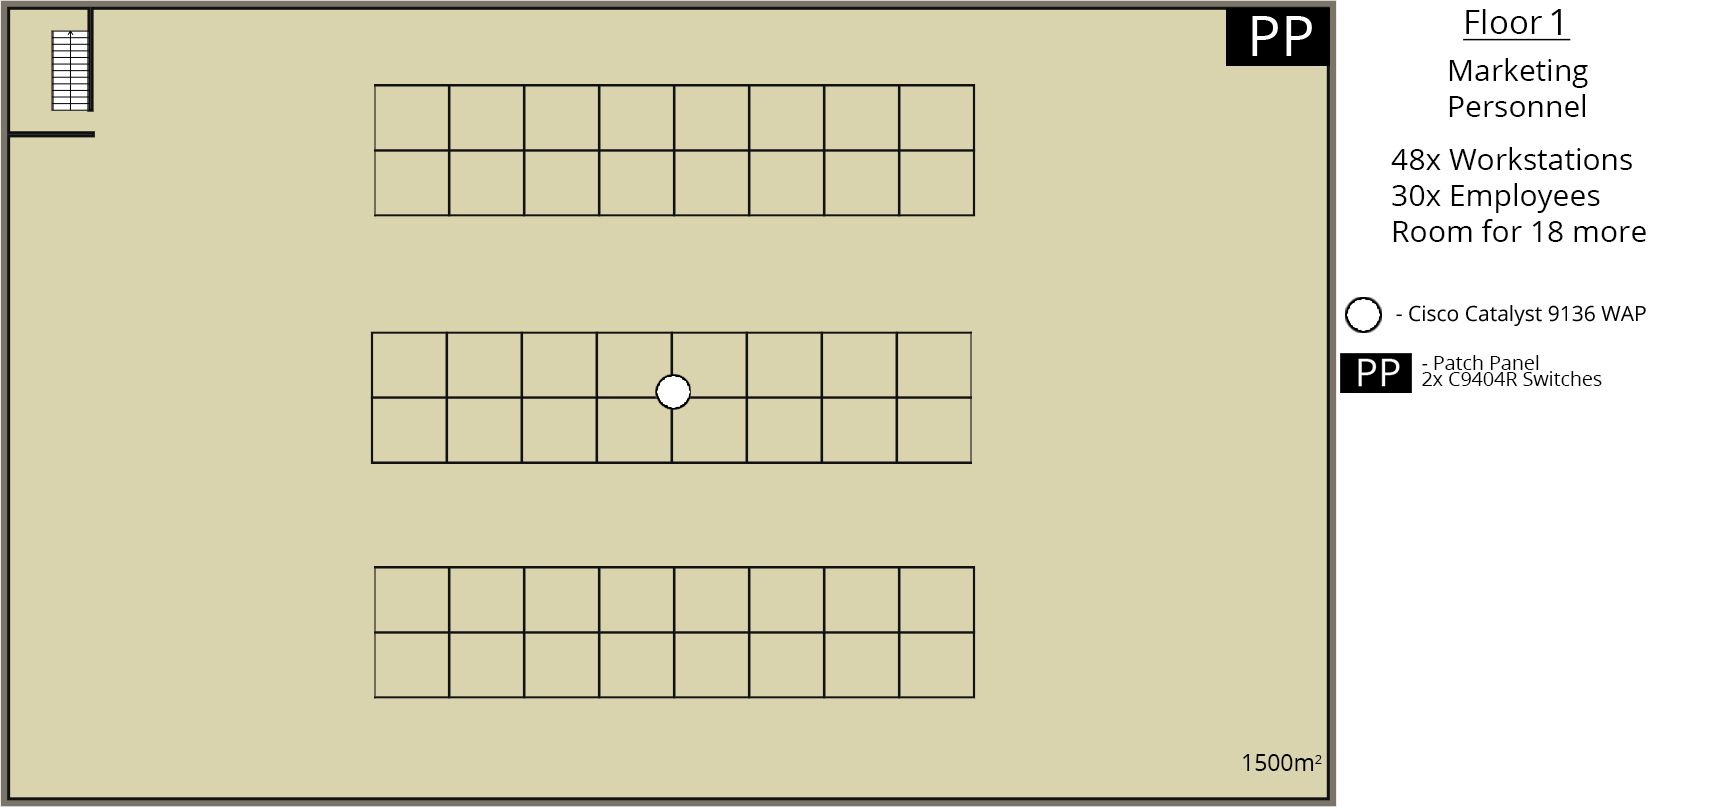
\includegraphics[width=15cm]{Figures/1st-floor.png}
    \caption{1st floor plan}
    \label{fig:1st_floor}
\end{figure}
\subsection{2nd Floor}
\begin{figure}[H]
    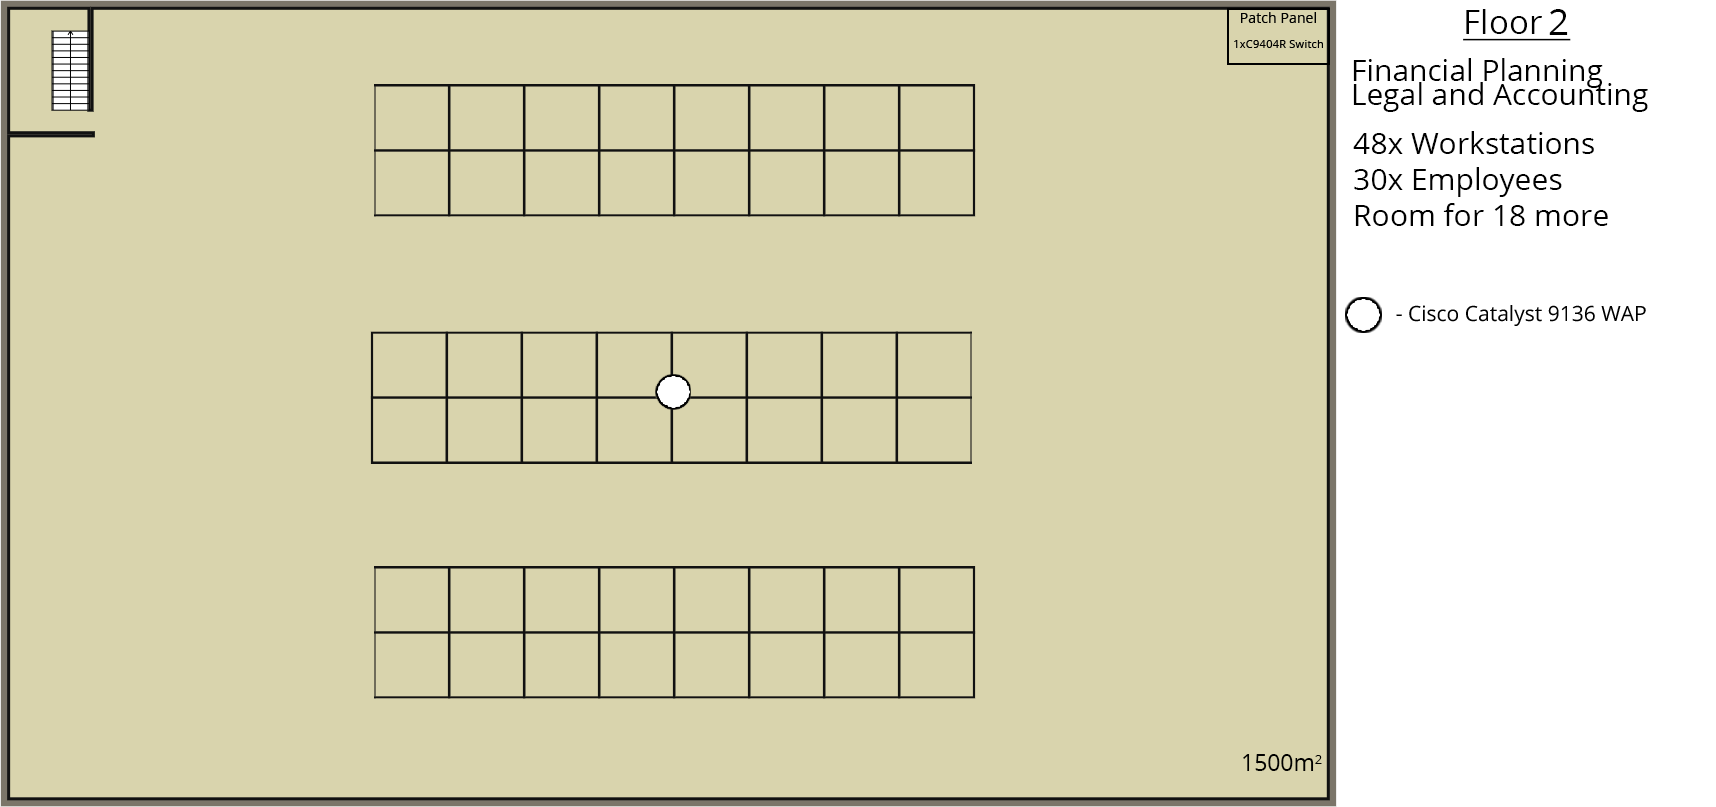
\includegraphics[width=15cm]{Figures/2nd-floor.png}
    \caption{2nd floor plan}
    \label{fig:2nd_floor}
\end{figure}
\subsection{3rd Floor}
\begin{figure}[H]
    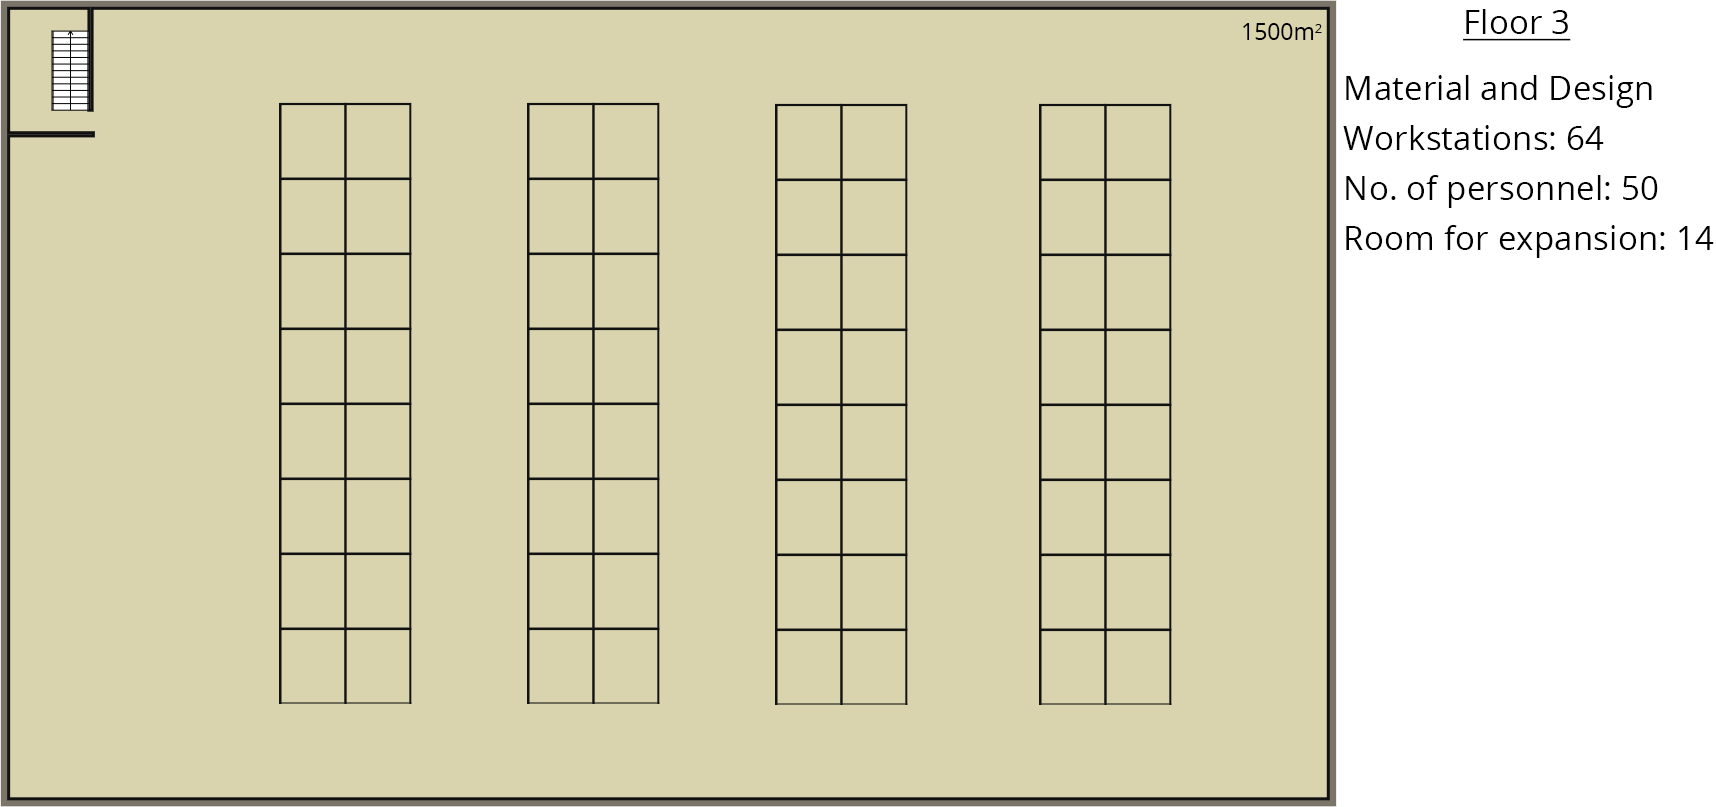
\includegraphics[width=15cm]{Figures/3rd-Floor.png}
    \caption{3rd floor plan}
    \label{fig:3rd_floor}
\end{figure}
\subsection{4th Floor}
\begin{figure}[H]
    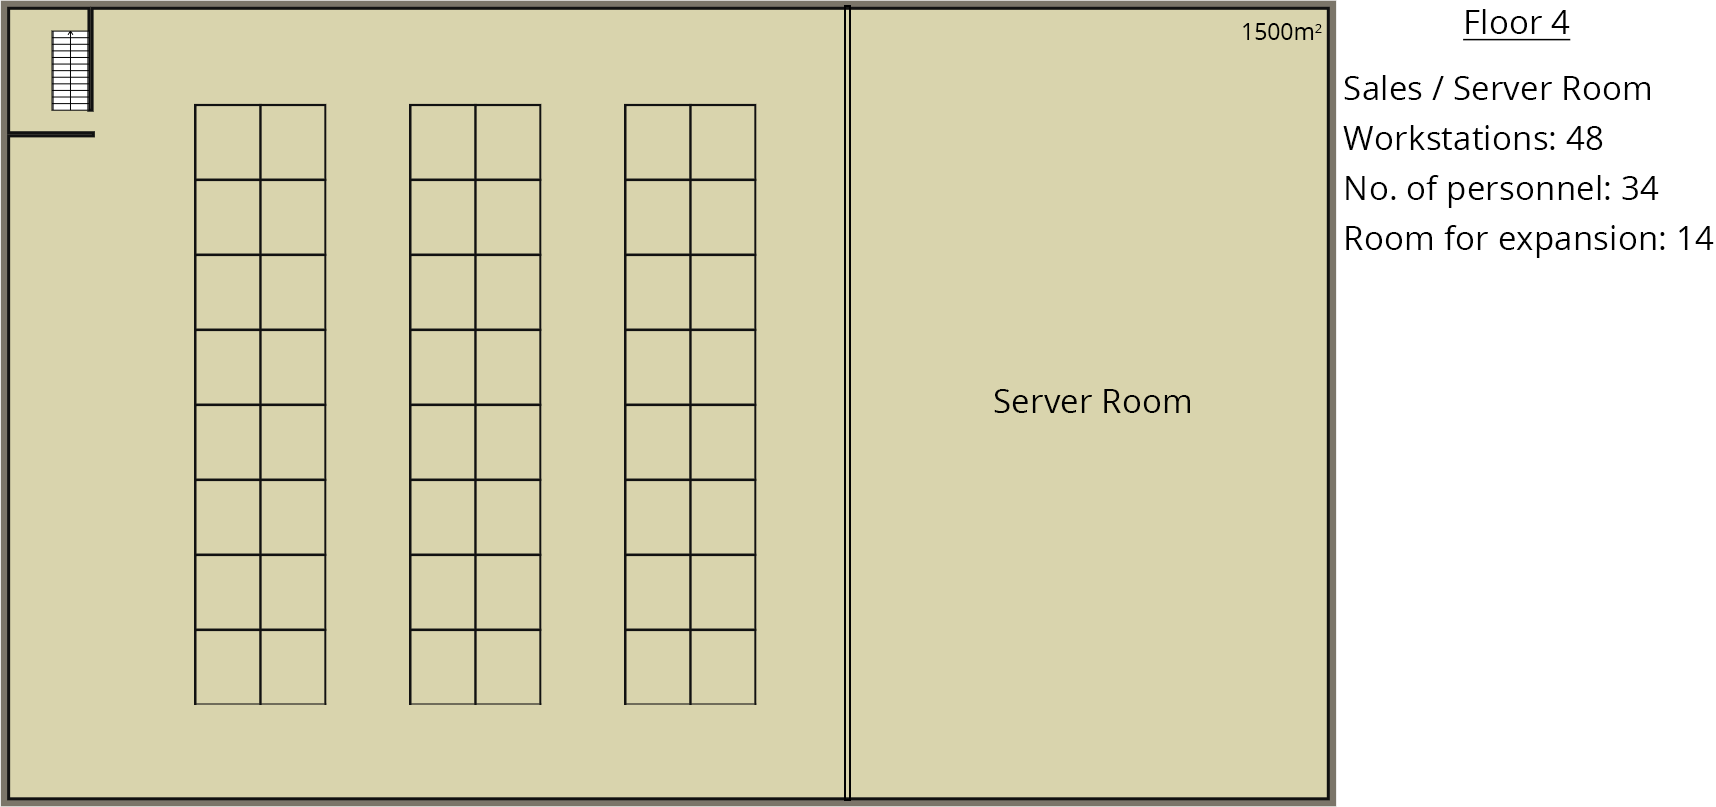
\includegraphics[width=15cm]{Figures/4th-Floor.png}
    \caption{4th floor plan}
    \label{fig:4th_floor}
\end{figure}
Explain why server room here
\subsection{5th Floor}
\begin{figure}[H]
    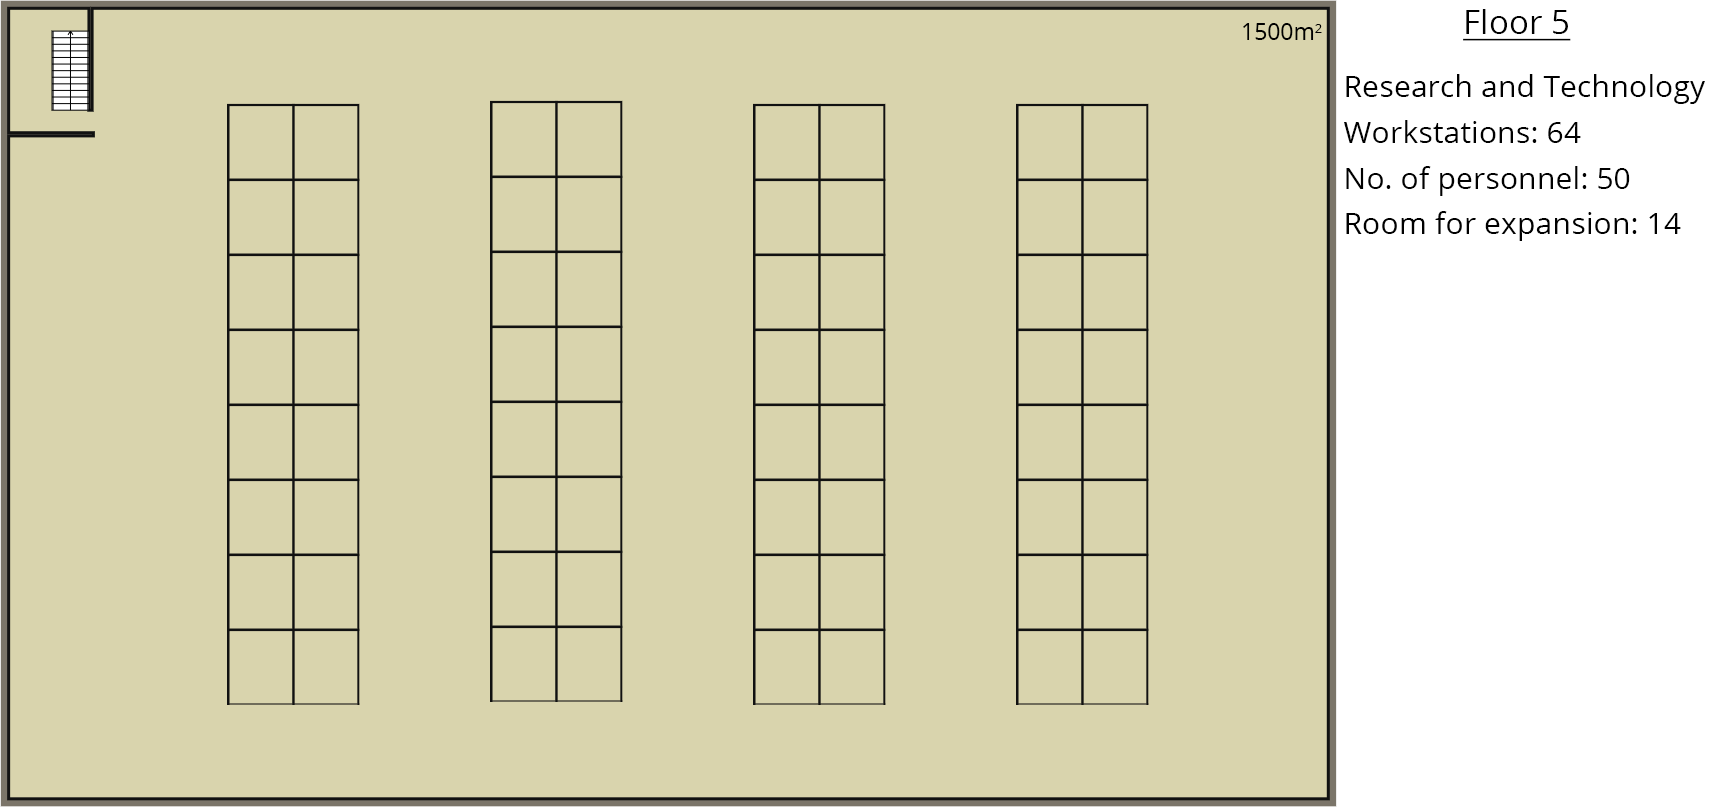
\includegraphics[width=15cm]{Figures/5th-Floor.png}
    \caption{5th floor plan}
    \label{fig:5th_floor}
\end{figure}
\subsection{6th Floor}
\begin{figure}[H]
    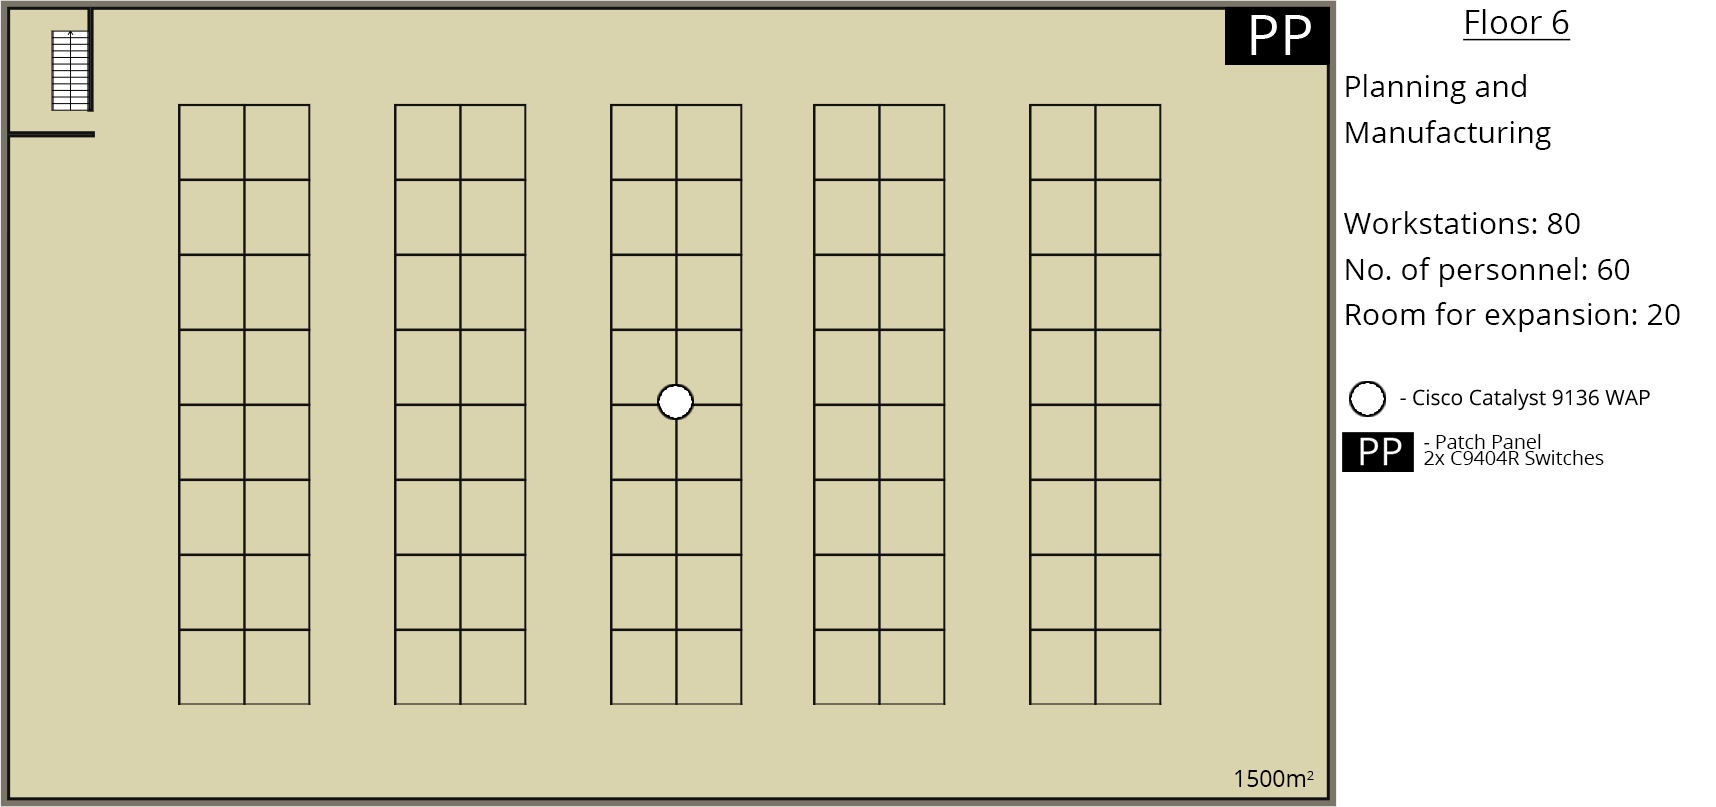
\includegraphics[width=15cm]{Figures/6th-Floor.png}
    \caption{6th floor plan}
    \label{fig:6th_floor}
\end{figure}
\subsection{7th Floor}
\begin{figure}[H]
    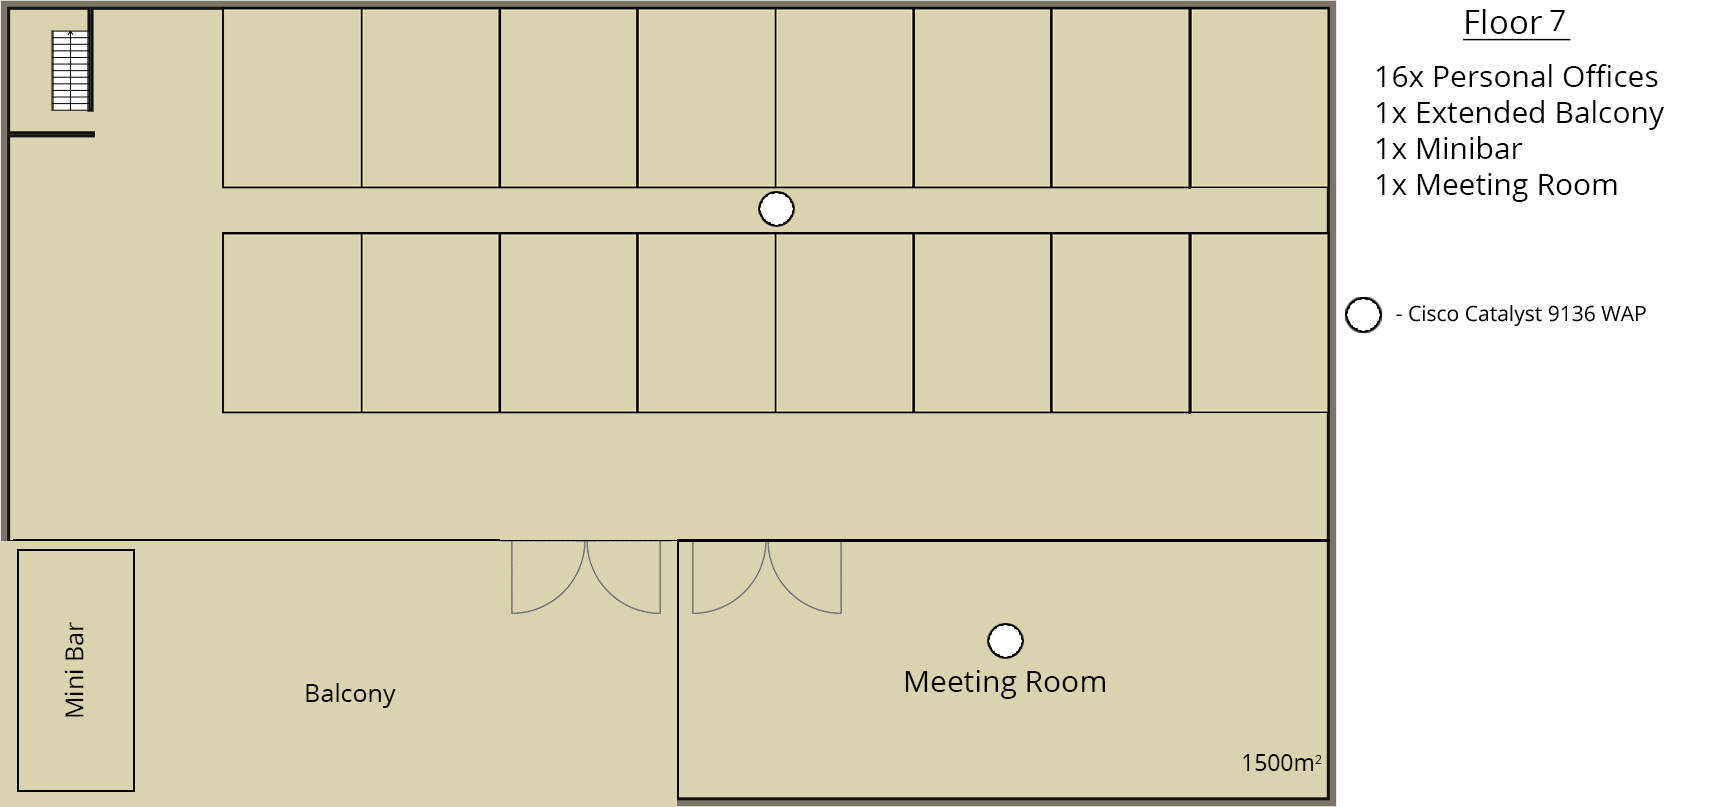
\includegraphics[width=15cm]{Figures/7th-floor.png}
    \caption{7th floor plan}
    \label{fig:7th_floor}
\end{figure}
\subsection{Server Room}
% \begin{figure}
%     \centering
%     \includegraphics[width=15cm]{Figures/}
%     \caption{Server racks diagram}
%     \label{fig:}
% \end{figure}